% Orange Pi Zero Family | Practical Embedded Linux Engineering Reference
% Generated 2026-10-11. Verify target board revision and image release before deployment.
\documentclass[10pt,oneside,openany]{report}
\usepackage[letterpaper,margin=0.78in,top=0.86in,bottom=0.82in,headheight=18pt]{geometry}
\usepackage[T1]{fontenc}
\usepackage[utf8]{inputenc}
% pdfLaTeX-only typography (migrated from fontspec): Noto Serif (roman) via
% the Type 1 "noto" package, Inter (sans) via its Type 1 package; DejaVu Sans
% Mono keeps its original 0.81 scaling.
\usepackage[rm]{noto}
\usepackage{inter}
\usepackage[scaled=0.81]{DejaVuSansMono}
\usepackage{microtype}
\emergencystretch=2em
\usepackage{amssymb}
\usepackage[table]{xcolor}
\definecolor{ink}{HTML}{152A3A}
\definecolor{navy}{HTML}{102E43}
\definecolor{teal}{HTML}{007E87}
\definecolor{copper}{HTML}{E8782C}
\definecolor{slate}{HTML}{506675}
\definecolor{paper}{HTML}{F3F8F9}
\definecolor{paleorange}{HTML}{FFF6EA}
\definecolor{linegray}{HTML}{D9E3E8}
\usepackage{xurl}
\usepackage{hyperref}
\hypersetup{colorlinks=true,linkcolor=teal,urlcolor=teal,citecolor=teal,pdftitle={Orange Pi Zero Family: Embedded Linux Engineering Guide},pdfauthor={Engineering Reference},pdfsubject={Hardware, Linux, GPIO, Docker, security and embedded systems labs}}
\usepackage{booktabs,tabularx,longtable,array,multirow}
\renewcommand{\arraystretch}{1.23}
\usepackage{enumitem}
\setlist[itemize]{leftmargin=1.45em,itemsep=2pt,topsep=4pt}
\setlist[enumerate]{leftmargin=1.55em,itemsep=3pt,topsep=4pt}
\usepackage{fancyhdr}
\pagestyle{fancy}\fancyhf{}
\fancyhead[L]{\sffamily\scriptsize\color{slate}ORANGE PI ZERO / ENGINEERING REFERENCE}
\fancyhead[R]{\sffamily\scriptsize\color{slate}\nouppercase{\leftmark}}
\fancyfoot[L]{\sffamily\scriptsize\color{slate}11 October 2026 \;\textbar\; v1.0}
\fancyfoot[R]{\sffamily\scriptsize\color{slate}\thepage}
\renewcommand{\headrulewidth}{0.3pt}
\renewcommand{\footrulewidth}{0pt}
\fancypagestyle{plain}{\fancyhf{}\fancyfoot[R]{\sffamily\scriptsize\color{slate}\thepage}\renewcommand{\headrulewidth}{0pt}}
\usepackage{titlesec}
\titleformat{\chapter}[display]{\sffamily\bfseries\color{navy}}{\fontsize{11}{13}\selectfont PART \thechapter}{5pt}{\fontsize{23}{26}\selectfont}
\titlespacing*{\chapter}{0pt}{-12pt}{18pt}
\titleformat{\section}{\sffamily\Large\bfseries\color{navy}}{\thesection}{0.7em}{}
\titleformat{\subsection}{\sffamily\large\bfseries\color{teal}}{\thesubsection}{0.65em}{}
\usepackage[most]{tcolorbox}
\newtcolorbox{fieldnote}[1][]{enhanced,breakable,frame hidden,boxrule=0pt,borderline west={2.5pt}{0pt}{teal},colback=paper,top=7pt,bottom=7pt,left=11pt,right=8pt,#1}
\newtcolorbox{cautionbox}[1][]{enhanced,breakable,frame hidden,boxrule=0pt,borderline west={2.5pt}{0pt}{copper},colback=paleorange,top=7pt,bottom=7pt,left=11pt,right=8pt,#1}
\usepackage{listings}
\lstdefinestyle{base}{basicstyle=\ttfamily\scriptsize,backgroundcolor=\color{paper},frame=single,framesep=7pt,rulecolor=\color{linegray},breaklines=true,breakatwhitespace=true,showstringspaces=false,tabsize=2,columns=fullflexible,keepspaces=true,upquote=true,aboveskip=8pt,belowskip=8pt}
\lstdefinestyle{sh}{style=base,language=bash,keywordstyle=\color{teal}\bfseries,commentstyle=\color{slate}\itshape}
\lstdefinestyle{python}{style=base,language=Python,keywordstyle=\color{teal}\bfseries,commentstyle=\color{slate}\itshape,stringstyle=\color{copper}}
\lstdefinestyle{config}{style=base}
\usepackage{tikz}
\usetikzlibrary{arrows.meta,positioning,shapes,fit,calc}
\usepackage{needspace}
\newcommand{\tagline}[1]{\noindent{\color{teal}\sffamily\bfseries\small\MakeUppercase{#1}}\par\medskip}
\newcommand{\code}[1]{\texttt{#1}}
\newcommand{\smallref}[1]{{\sffamily\scriptsize\color{slate}[#1]}}
\newcommand{\checkitem}{\(\square\)\;}
\begin{document}
\hypersetup{pageanchor=false}
\begin{titlepage}
\pagecolor{navy}\color{white}
\vspace*{0.60in}
{\color{copper}\sffamily\bfseries\fontsize{12}{16}\selectfont FIELD ENGINEERING / ARM SINGLE-BOARD COMPUTERS}\par
\vspace{0.5in}
{\sffamily\bfseries\fontsize{37}{41}\selectfont Orange Pi Zero\\[4pt]Engineering Guide}\par
\vspace{0.23in}
{\sffamily\fontsize{17}{22}\selectfont Hardware Architecture \textbullet\ Linux Deployment \\ GPIO \& Buses \textbullet\ Networking \textbullet\ Containers \textbullet\ Security}\par
\vspace{0.6in}

\begin{tikzpicture}[x=1cm,y=1cm]
  \draw[copper,line width=2.6pt] (0,0)--(12.6,0);
  \foreach \x/\a/\b in {0/BOOT/01,3.15/INTERFACE/02,6.30/DEPLOY/03,9.45/HARDEN/04}{
    \fill[white,opacity=.09] (\x,-1.45) rectangle ++(2.8,1.15);
    \node[anchor=west,font=\sffamily\bfseries\small,text=white] at (\x+.15,-.62) {\a};
    \node[anchor=east,font=\sffamily\tiny,text=copper] at (\x+2.63,-1.20) {\b};
  }
\end{tikzpicture}
\vfill
{\sffamily\large Technical Reference and Lab Workbook}\par
{\sffamily\small Covering Zero / LTS, Zero 2W, Zero 3, Zero 3W and Zero 4}\par\vspace{9pt}
{\sffamily\small Version 1.0 \textbar\ 11 October 2026}\par
\end{titlepage}
\hypersetup{pageanchor=true}
\nopagecolor\color{ink}
\pagenumbering{roman}
\chapter*{How to use this guide}
\addcontentsline{toc}{chapter}{How to use this guide}
This document is a \emph{practical, architecture-first engineering guide}, not a substitute for the silkscreen, schematic, revision-specific user manual, or image release notes. Orange Pi uses different system-on-chips (SoCs), boot firmware, pin multiplexing and kernel-support paths across the ``Zero'' name. Apply a procedure only after matching the exact board revision and the operating-system image.
\begin{fieldnote}
\textbf{Fast path.} Identify the board (Chapter 1), choose a supported image (Chapter 3), provision with console recovery (Chapter 4), configure networking (Chapter 5), harden SSH before exposing a service (Chapter 9), and then select a project lab (Chapter 10). Code examples are reference implementations: adapt GPIO offsets, interfaces and IP addresses to measured hardware.
\end{fieldnote}
\textbf{Conventions.} Lines prefixed \code{sudo} require administrative authority. Angle-bracket placeholders denote values to replace. Shell examples assume a Debian/Ubuntu-style user space. \textbf{Do not copy a sample block-device path, pin number, or IP address without verifying it.}
\begin{cautionbox}
\textbf{Electrical and operational safety.} The GPIO domain is generally 3.3\,V logic. Never apply 5\,V to a signal pin, connect mains voltage to the board, directly switch inductive loads with GPIO, or connect an RS-232 serial adapter to a TTL UART. Power off before rewiring. Use appropriate fusing, level shifting and isolation. Treat first-boot passwords and externally published container ports as security-critical.
\end{cautionbox}
\tableofcontents
\clearpage
\pagenumbering{arabic}

\chapter{Portfolio and hardware selection}
\section{Model differentiation}
\begin{center}
\small\begin{tabularx}{\textwidth}{@{}p{2.45cm}p{2.45cm}p{2.0cm}X@{}}\toprule
\textbf{Board} & \textbf{CPU / ISA} & \textbf{RAM class} & \textbf{Design implications}\\\midrule
Original Zero / LTS & H2+ or H3; 4\(\times\) Cortex-A7, ARMv7 (32-bit) & 256/512 MB DDR3 & 100 MbE and older wireless; very lean headless services; limited RAM and armhf user space.\\
Zero 2W & H618; 4\(\times\) Cortex-A53, ARMv8 & 1--4 GB LPDDR4 & Very small wireless-focused form factor; Ethernet requires compatible expansion/adapter.\\
Zero 3 & H618; 4\(\times\) Cortex-A53, ARMv8 & 1/1.5/2/4 GB LPDDR4 & Built-in Gigabit Ethernet, Wi-Fi 5, 26-pin plus secondary expansion.\\
Zero 3W & A733; 2\(\times\) A76 + 6\(\times\) A55 & Up to 16 GB LPDDR5 & 40-pin header, Wi-Fi 6, optional storage/PCIe connectivity; \emph{no onboard RJ45}.\\
Zero 4 & A733; 2\(\times\) A76 + 6\(\times\) A55 & Up to 16 GB* & Onboard Gigabit Ethernet; different layout from 3W; PCIe/USB expansion with adapter constraints.\\\bottomrule
\end{tabularx}
\end{center}
{\footnotesize *Maximum advertised platform capability is not a guarantee of a specific purchasable configuration. A733 GPU/NPU, display, PCIe and other peripheral enablement depends on image/driver availability. Sources: [1]--[5], [16].}\par
\section{Architecture and practical selection}
The original 32-bit board is appropriate for a DNS forwarder, logging endpoint or microcontroller gateway but is constrained for multi-container applications. The H618 models are practical \code{arm64} Linux nodes; the Zero 3 is the simpler wired appliance. A733 boards add large memory and heterogeneous compute, but kernel ABI, DTB, graphics and accelerator maturity must be verified before a production commitment.
\begin{center}
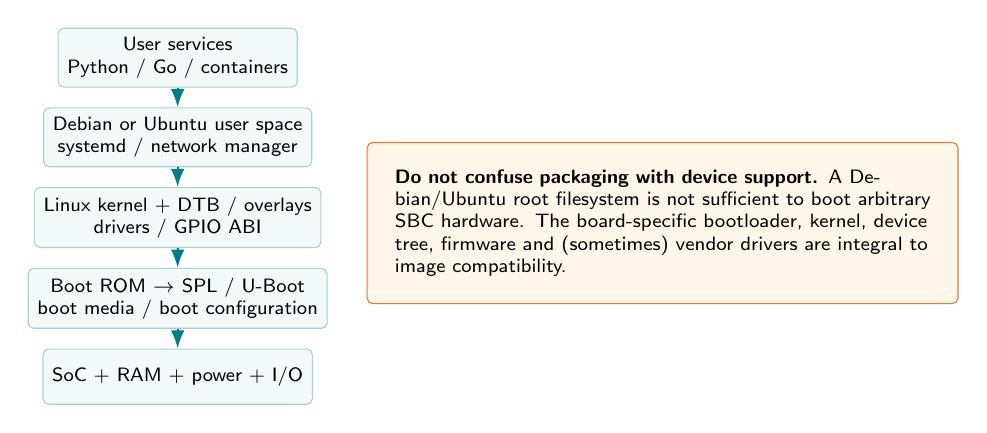
\begin{tikzpicture}[font=\sffamily\scriptsize,>=Latex,node distance=0.25cm]
\tikzstyle{part}=[draw=teal!35,fill=paper,rounded corners=2pt,minimum height=.7cm,align=center]
\node[part,minimum width=3.0cm] (app) {User services\\Python / Go / containers};
\node[part,minimum width=3.0cm,below=of app] (os) {Debian or Ubuntu user space\\systemd / network manager};
\node[part,minimum width=3.0cm,below=of os] (kernel) {Linux kernel + DTB / overlays\\drivers / GPIO ABI};
\node[part,minimum width=3.0cm,below=of kernel] (boot) {Boot ROM \(\to\) SPL / U-Boot\\boot media / boot configuration};
\node[part,minimum width=3.0cm,below=of boot] (hw) {SoC + RAM + power + I/O};
\draw[->,teal,thick] (app)--(os);\draw[->,teal,thick] (os)--(kernel);\draw[->,teal,thick] (kernel)--(boot);\draw[->,teal,thick] (boot)--(hw);
\node[draw=copper,rounded corners=2pt,fill=paleorange,align=left,anchor=west,text width=6.8cm,inner sep=10pt] at (2.4,-2.1) {\textbf{Do not confuse packaging with device support.} A Debian/Ubuntu root filesystem is not sufficient to boot arbitrary SBC hardware. The board-specific bootloader, kernel, device tree, firmware and (sometimes) vendor drivers are integral to image compatibility.};
\end{tikzpicture}
\end{center}
\section{Hardware acceptance checklist}
\begin{itemize}
\item \checkitem Photograph front/back, identify exact silkscreen/revision, SoC and RAM size.
\item \checkitem Obtain the matching official pinout and user manual; record header pin 1 orientation.
\item \checkitem Inventory USB OTG/host roles, Ethernet connector, serial debug header, Wi-Fi antenna, microSD and internal storage provisioning.
\item \checkitem Confirm supply voltage/current and connector polarity per revision; select a short, adequately sized cable.
\item \checkitem Verify the intended image supports required Wi-Fi, SPI/I\(^{2}\)C, PWM, camera, display and watchdog features \emph{on that specific build}.
\end{itemize}
\section{Power, thermals and storage reliability}
For a conservative A733 development station, use the documented 5\,V/3\,A USB-C source; do not assume that power rating applies to all earlier boards. USB peripherals, expansion boards and startup transients add demand. Monitor \code{dmesg}, reboot count, \code{/sys/class/thermal}, CPU throttling and filesystem errors. Avoid using a cheap SD card for a high-write database or logging system; select an endurance-rated card or supported internal storage. Plan backup/restoration before migrating boot media.

\chapter{Boot architecture and peripheral discovery}
\section{Boot chain and board support package}
A typical Allwinner Linux boot path is SoC boot ROM \(\rightarrow\) initial loader/DRAM initialization \(\rightarrow\) U-Boot \(\rightarrow\) Linux kernel + device-tree blob (DTB) \(\rightarrow\) initramfs/root filesystem \(\rightarrow\) \code{systemd}. Exact media priority and loader layout vary by SoC and image. The DTB binds hardware controllers, clock trees and pin mux to drivers; an incorrect DTB can yield absent GPIO buses or a nonbooting board.
\begin{lstlisting}[style=sh]
# Discover actual hardware, kernel and boot configuration.
cat /proc/device-tree/model 2>/dev/null; echo
tr '\0' '\n' </proc/device-tree/compatible 2>/dev/null
uname -a
cat /etc/os-release
lsblk -o NAME,SIZE,TYPE,FSTYPE,MOUNTPOINTS,MODEL
find /boot -maxdepth 2 \( -name 'armbianEnv.txt' -o -name '*.dtb' \) \
  2>/dev/null | head -40
\end{lstlisting}
\section{Kernel drivers versus GPIO bit-banging}
Use dedicated kernel interfaces where present: \code{/dev/i2c-*} for I\(^{2}\)C, \code{/dev/spidev*} for SPI, \code{/dev/ttyS*} for serial and \code{/dev/gpiochip*} for unclaimed digital lines. Do not manually control a bus through raw GPIO when an in-kernel controller driver is available. Prefer the GPIO character-device ABI v2 over the obsolete sysfs \code{/sys/class/gpio} method. \smallref{[7],[8]}
\begin{lstlisting}[style=sh]
ls -l /dev/gpiochip* /dev/i2c-* /dev/spidev* /dev/ttyS* 2>/dev/null
sudo apt update
sudo apt install -y gpiod i2c-tools usbutils pciutils ethtool
command -v gpioinfo && gpioinfo
sudo dmesg | grep -Ei 'gpio|pinctrl|i2c|spi|mmc|eth|wifi' | tail -70
\end{lstlisting}
\begin{cautionbox}
Pin numbers printed on the 26- or 40-position header are \emph{physical} connector positions. Linux GPIO chip offsets, Allwinner port names (for example \code{PH6}) and physical positions are three different numbering systems. Never substitute one for another. Pinmux functions are mutually exclusive on a given pad.
\end{cautionbox}

\chapter{Operating-system selection and lifecycle}
\section{Armbian, vendor Debian and vendor Ubuntu}
Armbian supplies board-specific kernels, bootloaders, DTBs and tooling over Debian/Ubuntu user spaces. Vendor images may enable unusual board peripherals earlier, but often require tracking downstream kernel trees, build provenance, CVE handling and update commitments. Generic ARM64 server installers are \emph{not} interchangeable with board images. \smallref{[6],[9]}
\begin{center}\small\begin{tabularx}{\textwidth}{@{}p{2.35cm}X X@{}}\toprule
\textbf{Choice} & \textbf{Advantages} & \textbf{Trade-offs / verification}\\\midrule
Armbian Debian minimal & Low idle footprint; standard APT; useful for appliances & Support status varies: community builds can be automated/untested; kernel branch matters.\\
Armbian Ubuntu server & Familiar packaging and toolchain; SBC configuration utility & Some boards have no server variant; inspect available image, date and branch.\\
Orange Pi vendor image & Board-specific peripheral enablement and reference configuration & Document vendor kernel lineage, package security fixes and upgrade/restore plan.\\
Self-built Armbian & Reproducible feature selection, patched kernels and overlays & Requires build validation, artifact signing and regression testing.\\\bottomrule\end{tabularx}\end{center}
\section{Support snapshot: 11 October 2026}
Armbian lists the original Zero, Zero 2W and Zero 3 as \emph{community} targets. The Zero 3W appears as a \emph{standard} target with vendor-kernel images. The public board list did not establish equivalent ready-to-use Zero 4 support at the time of research: treat Zero 4 image selection as a separate validation step. Images, support levels and kernel versions change; refer to each linked board page immediately before flashing. \smallref{[10]--[13]}
\begin{fieldnote}
\textbf{Release selection rule.} Choose a board-exact image with a documented release date, kernel branch, supported boot target and checksum. For deployment stability, prefer a tested release over a rolling image unless the latter is required to enable hardware. Record the filename, SHA-256 digest, provenance and recovery media.
\end{fieldnote}
\section{Reproducible image decision record}
\begin{center}\small\begin{tabularx}{\textwidth}{@{}p{3.6cm}X@{}}\toprule
\textbf{Attribute} & \textbf{Record before deployment}\\\midrule
Exact model and PCB revision & \rule{0pt}{2.1ex}\dotfill\\
Image name / SHA-256 / source URL & \dotfill\\
Bootloader / kernel / DTB branch & \dotfill\\
Supported Ethernet / Wi-Fi / I\(^{2}\)C / SPI & \dotfill\\
Patch/update owner and recovery plan & \dotfill\\\bottomrule\end{tabularx}\end{center}

\chapter{Provisioning and Linux installation}
\section{Prepare the development workstation}
You need a board-specific image, a quality microSD card, a capable power adapter, a USB-to-UART \emph{3.3\,V TTL} debug adapter if supported, an Ethernet cable where applicable and access to the router's DHCP leases. Armbian recommends its Imager to select/download/write images; it also recommends suitable A1/A2 media. \smallref{[9]}
\begin{lstlisting}[style=sh]
# Linux workstation, NOT the Orange Pi: verify the image and target.
sha256sum OrangePi-image.img.xz
lsblk -o NAME,SIZE,MODEL,TRAN,MOUNTPOINTS
# Compare the checksum with the publisher's authenticated digest.
# SAFER: flash with Armbian Imager or Balena Etcher and verify.
\end{lstlisting}
For an expert-only \code{dd} workflow, \textbf{explicitly identify the removable device} before running and ensure that it is not a mounted partition or host disk. This operation overwrites the entire target.
\begin{lstlisting}[style=sh]
# EXAMPLE ONLY -- replace /dev/sdX after confirming lsblk twice.
# umount any partitions of the chosen removable device first.
xzcat OrangePi-image.img.xz | sudo dd of=/dev/sdX \
  bs=4M status=progress conv=fsync
sync
\end{lstlisting}
\section{First boot procedure}
\begin{enumerate}
\item Insert flashed media with power disconnected; attach serial console (when available) and Ethernet before power.
\item Boot with an adequate supply; inspect the kernel console or DHCP reservations for an assigned address.
\item Follow the \emph{image-specific} first-login workflow. Armbian commonly starts with a temporary \code{root} / \code{1234} SSH credential and forces its replacement; do not leave it active. \smallref{[14]}
\item Create an unprivileged admin identity, select locale/timezone, install your SSH public key and update packages.
\item Save a baseline inventory before changing overlays, network routes or boot media.
\end{enumerate}
\begin{lstlisting}[style=sh]
hostnamectl
ip -brief address
ip route
sudo apt update && sudo apt full-upgrade -y
sudo reboot
# after reboot
uptime
systemctl --failed
journalctl -b -p warning --no-pager | tail -50
\end{lstlisting}
\section{Debian/Ubuntu application baseline}
\begin{lstlisting}[style=sh]
sudo apt install -y ca-certificates curl git vim tmux jq \
  htop iotop sysstat dnsutils iproute2 rsync chrony \
  python3 python3-venv python3-pip
sudo timedatectl set-timezone America/New_York
systemctl status chrony --no-pager
cat /etc/os-release; dpkg --print-architecture
\end{lstlisting}
Run \code{armbian-config} when using Armbian for supported network, storage, kernel and hardware options. Avoid copying outdated overlay names across SoCs. Internal-media migration is destructive if aimed at the wrong block device; retain known-good microSD recovery media. \smallref{[15]}
\section{Rescue and rollback planning}
Keep a second verified card with a known-good image, a current backup of \code{/etc}, SSH keys securely stored off-device, and a working serial console. Before a kernel, U-Boot or DTB change, record \code{uname -a}, installed packages, \code{/boot} files and the previous image. A release upgrade is a \emph{hardware regression event}: test network, serial, storage and all connected buses after reboot.

\chapter{Networking and remote operations}
\section{Know the network manager before changing it}
Armbian variants may use NetworkManager, Netplan with a selected renderer, or \code{systemd-networkd}. Do not install a second network manager or simultaneously edit conflicting config sources. On a headless SBC, prefer router-side DHCP address reservations to a static address; preserve console access before editing the active NIC. \smallref{[15]}
\begin{lstlisting}[style=sh]
ip -br link
ip -br address
ip route show
resolvectl status || cat /etc/resolv.conf
systemctl is-active NetworkManager systemd-networkd
nmcli device status 2>/dev/null || true
networkctl status --no-pager 2>/dev/null || true
\end{lstlisting}
\section{NetworkManager recipes (where active)}
\begin{lstlisting}[style=sh]
# List actual interfaces and connection names; do not assume eth0.
nmcli -f DEVICE,TYPE,STATE,CONNECTION dev status
nmcli connection show
# Interactive Wi-Fi connection: avoid credentials in shell history.
sudo nmcli --ask dev wifi connect 'YOUR_SSID' ifname wlan0
# Example DHCP refresh on an existing NetworkManager profile:
sudo nmcli connection up 'Wired connection 1'
\end{lstlisting}
For IPv4 static configuration, record the active profile, gateway, resolver and management subnet first. Then set \code{ipv4.method manual}, address, gateway and DNS on the verified profile. NetworkManager can recover a lost connection through serial console; never rely on a blind remote network migration.
\section{Connectivity verification and port exposure}
\begin{lstlisting}[style=sh]
ping -c 3 1.1.1.1
getent ahostsv4 debian.org
resolvectl query debian.org || true
ss -tulpen
sudo ethtool eth0 2>/dev/null | grep -E 'Speed:|Link detected:'
# Replace the host IP with the actual DHCP or reserved address.
ssh -o StrictHostKeyChecking=ask admin@192.0.2.10
\end{lstlisting}
Example address \code{192.0.2.10} is documentation-only, not a usable LAN address. Bind development services to \code{127.0.0.1} and use an SSH tunnel for off-device access:
\begin{lstlisting}[style=sh]
# Workstation: forward local port 8080 to a service on the board.
ssh -L 8080:127.0.0.1:8080 admin@<board-lan-ip>
\end{lstlisting}
\section{Network topology and segmentation}
\begin{center}
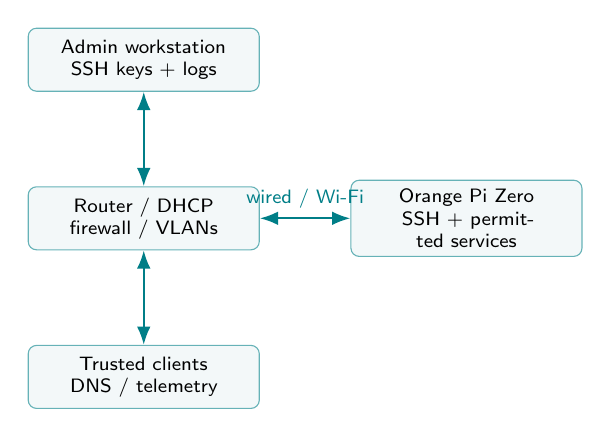
\begin{tikzpicture}[node distance=1.2cm and 1.15cm,font=\sffamily\scriptsize,>=Latex]
\tikzstyle{n}=[draw=teal!60,fill=paper,rounded corners=3pt,minimum height=.8cm,text width=2.7cm,align=center]
\node[n] (router) {Router / DHCP\\firewall / VLANs};
\node[n,right=of router] (pi) {Orange Pi Zero\\SSH + permitted services};
\node[n,above=of router] (laptop) {Admin workstation\\SSH keys + logs};
\node[n,below=of router] (lan) {Trusted clients\\DNS / telemetry};
\draw[<->,thick,teal] (router)--node[above]{wired / Wi-Fi}(pi);
\draw[<->,thick,teal] (router)--(laptop);
\draw[<->,thick,teal] (router)--(lan);
\end{tikzpicture}
\end{center}
A defensible deployment separates device management from client-facing traffic, blocks inbound WAN access by default, and explicitly enumerates allowed protocols and ports. Do not expose SSH, Docker daemon APIs, MQTT without authentication, or a DNS resolver to the public internet.

\chapter{GPIO, I2C, SPI and UART}
\section{Connector and electrical discipline}
The physical header is \emph{not} a universal Raspberry Pi-compatible electrical contract. Orange Pi Zero 3W exposes a 40-pin header; Zero 3 and Zero 4 use different headers and peripheral routing. Even when connector dimensions match, pin functions, regulator capabilities and available kernel drivers may not. Acquire the exact manufacturer's pinout before every circuit. \smallref{[1]--[5]}
\begin{center}\small\begin{tabularx}{\textwidth}{@{}p{1.2cm}p{3.1cm}X@{}}\toprule
\textbf{Bus} & \textbf{Linux userspace} & \textbf{Design considerations}\\\midrule
GPIO & \code{/dev/gpiochipN}, libgpiod & Confirm chip/offset/pinmux; avoid 5\,V; set direction and safe startup state.\\
I\(^{2}\)C & \code{/dev/i2c-N}, smbus2 & Shared SCL/SDA, compatible bus voltage, pull-up sizing and unique 7-bit addresses.\\
SPI & \code{/dev/spidevB.C} & MOSI/MISO/SCLK/CS and mode; separate chip select; limited cable length.\\
UART & \code{/dev/ttyS*} or equivalent & 3.3\,V TTL levels, matching baud/ground, RX\(\leftrightarrow\)TX; avoid console conflicts.\\
PWM & pwmchip or appropriate driver & Kernel and overlay maturity varies; never assume a PWM pin is available.\\\bottomrule\end{tabularx}\end{center}
\begin{cautionbox}
\textbf{Protect the board.} Connect GPIO \(\to\) series resistor \(\to\) LED \(\to\) ground only after identifying the correct pin and polarity. A 330--1,000\,\(\Omega\) series resistor is reasonable for a basic 3.3\,V indicator LED, subject to the LED's voltage and the SoC pin current limit. For relays, solenoids and motors use a driver transistor/MOSFET, flyback protection and an appropriately isolated power path.
\end{cautionbox}
\section{Device-tree overlays and pin multiplexing}
Kernel device trees specify which pads belong to SPI, UART, I\(^{2}\)C or another driver. On supported Armbian builds, open \code{sudo armbian-config} and inspect the kernel/device-tree overlay menu; exact overlay names are board- and kernel-dependent. Verify the resulting device node \emph{after reboot}. Keep a serial/SD recovery path before altering DTBs. \smallref{[17]}
\begin{lstlisting}[style=sh]
# Inspect, then enable only a board-specific documented overlay.
cat /boot/armbianEnv.txt 2>/dev/null || true
find /boot -type f \( -name '*.dtbo' -o -name '*.dtb' \) | head -40
sudo armbian-config
# After a controlled reboot:
ls /dev/i2c-* /dev/spidev* /dev/ttyS* 2>/dev/null
\end{lstlisting}
\section{Map header pads to Linux line offsets}
\begin{enumerate}
\item Locate physical pin 1 and the pad's signal label using the \emph{exact} pinout.
\item Read the SoC GPIO port/pad designation and verify the intended alternate function.
\item Inspect \code{gpioinfo} and any \code{line-name} mapping; read DTB pinctrl definitions where names are missing.
\item Record the observed \code{/dev/gpiochipN} and \emph{offset} and ensure no kernel consumer owns the line.
\item With wiring disconnected, request the output at a safe inactive level, then connect a current-limited test circuit.
\end{enumerate}
\begin{fieldnote}
\textbf{Portable practice.} Do not publish a hardcoded ``pin 7 = GPIO 4'' mapping across the Orange Pi Zero family. Maintain a small board-revision mapping file in the deployment repository, together with the pinout source, voltage domain and verified kernel version.
\end{fieldnote}
\section{Digital output with the libgpiod v2 Python API}
The following deliberately requires explicit chip and offset configuration to prevent implicit Raspberry Pi pin-number assumptions. \textbf{Install a Python binding compatible with libgpiod 2.x}; older Debian images may include a different 1.x binding/API. The line must not already be assigned to another driver. \smallref{[7],[18]}
\begin{lstlisting}[style=python]
#!/usr/bin/env python3
# led.py -- libgpiod 2.x only; requires GPIO_CHIP and GPIO_OFFSET.
import os
import time
import gpiod
from gpiod.line import Direction, Value

chip = os.environ["GPIO_CHIP"]          # e.g. /dev/gpiochip0
line = int(os.environ["GPIO_OFFSET"])  # actual line offset, not header pin

settings = gpiod.LineSettings(
    direction=Direction.OUTPUT, output_value=Value.INACTIVE
)
with gpiod.request_lines(
    chip, consumer="opi-led-lab", config={line: settings}
) as request:
    for _ in range(5):
        request.set_value(line, Value.ACTIVE)
        time.sleep(0.5)
        request.set_value(line, Value.INACTIVE)
        time.sleep(0.5)
\end{lstlisting}
\begin{lstlisting}[style=sh]
python3 -c 'import gpiod; print(gpiod.__file__)'
# Only after recording actual board mapping:
GPIO_CHIP=/dev/gpiochip0 GPIO_OFFSET=<verified-offset> \
  python3 led.py
\end{lstlisting}
\section{I2C discovery and bus safety}
\begin{lstlisting}[style=sh]
sudo apt install -y i2c-tools
ls -l /dev/i2c-*
i2cdetect -l
# Replace 1 with a VERIFIED bus index; scan can affect some devices.
sudo i2cdetect -y 1
\end{lstlisting}
Treat an I\(^{2}\)C address scan as a debugging technique, not a guaranteed harmless probe: certain devices react to SMBus commands. Confirm sensor supply voltage and pull-ups. A 5\,V-powered breakout may pull SDA/SCL above safe GPIO voltage unless it includes appropriate level shifting. The interface numbering is enumerated at boot and must be discovered, not guessed. \smallref{[19]}
\section{SPI and UART bring-up}
\begin{lstlisting}[style=sh]
# SPI nodes only appear after driver/overlay configuration.
ls -l /dev/spidev*
# Serial discovery and debug, not a mandate to use ttyS0:
find /dev -maxdepth 1 -name 'ttyS*' -o -name 'ttyUSB*'
sudo dmesg | grep -iE 'serial|uart|ttyS' | tail -25
# Install userspace serial tooling if needed:
sudo apt install -y minicom
\end{lstlisting}
Configure UART 8N1 and the device's baud rate; on a login console UART, first change the boot/login configuration to prevent collision. Use \emph{three-wire TTL} ground/TX/RX at compatible voltage; do not connect a standard RS-232 DB9 cable directly. Use physical SPI/I\(^{2}\)C modules rather than software emulation for reliable throughput.

\chapter{Process management, observability and performance}
\section{systemd service lifecycle}
A long-running embedded application should run as a dedicated non-root user, have an explicit working directory, restart policy, journaling and declared resource dependencies. Do not put custom code in privileged boot scripts. Example service for a Python application installed in \code{/opt/opi-app}:
\begin{lstlisting}[style=config]
# /etc/systemd/system/opi-app.service
[Unit]
Description=Orange Pi application
After=network-online.target
Wants=network-online.target

[Service]
Type=simple
User=opiapp
Group=opiapp
WorkingDirectory=/opt/opi-app
ExecStart=/opt/opi-app/.venv/bin/python /opt/opi-app/main.py
Restart=on-failure
RestartSec=5
NoNewPrivileges=true
ProtectSystem=strict
ProtectHome=true
PrivateTmp=true
StateDirectory=opi-app

[Install]
WantedBy=multi-user.target
\end{lstlisting}
\begin{lstlisting}[style=sh]
# Create the user and program directory before enabling the service.
sudo useradd --system --home /nonexistent --shell /usr/sbin/nologin opiapp
sudo install -d -o root -g root -m 0755 /opt/opi-app
sudo systemctl daemon-reload
sudo systemctl enable --now opi-app.service
systemctl status opi-app.service --no-pager
journalctl -u opi-app -b --no-pager -n 60
\end{lstlisting}
If the application writes files, place them under \code{/var/lib/opi-app} (supplied by \code{StateDirectory=}) rather than the read-only installation directory. If a service needs GPIO/I\(^{2}\)C, grant narrowly scoped device/group access; do not simply run it as root or chmod all devices to 777.
\section{Operational telemetry}
\begin{lstlisting}[style=sh]
free -h; df -hT; lsblk -f
vmstat 1 5
uptime
systemd-analyze blame | head -20
journalctl --disk-usage
cat /proc/loadavg
for z in /sys/class/thermal/thermal_zone*/temp; do \
  echo "$z: $(cat "$z") millidegrees C"; done
\end{lstlisting}
On embedded boards, a CPU thermal reading can be inaccurate for specific revisions; compare with external instruments when troubleshooting. Export CPU/RAM/disk/thermal metrics for long-running deployments. Enable log rotation, quantify SD-card write amplification, and monitor boot success, filesystem read-only remounts and watchdog resets.
\section{Backup and disaster recovery}
Use an \emph{image} for bootability and a separate file-level backup for configuration and data. Power down and image the SD card on a workstation for reliable bare-metal recovery. Also archive key configuration: \code{/etc}, application deployment descriptors, \code{/var/lib/<service>}, and package manifests. Encrypt backups containing SSH credentials or service secrets.
\begin{lstlisting}[style=sh]
mkdir -p "$HOME/backup-manifest"
dpkg-query -W > "$HOME/backup-manifest/packages.txt"
systemctl list-unit-files --state=enabled > \
  "$HOME/backup-manifest/enabled-units.txt"
uname -a > "$HOME/backup-manifest/kernel.txt"
# Test recovery on spare media, not merely successful backup creation.
\end{lstlisting}

\chapter{Containers and Docker Compose}
\section{Eligibility and installation}
Containers share the host kernel; they do not repair absent device drivers or mismatched CPU architecture. Inspect \code{uname -m}, \code{dpkg --print-architecture} and free memory before selecting packages. For low-memory 32-bit Zero boards, prefer native daemons; use only explicitly compatible \code{linux/arm/v7} images where required. On newer 64-bit SoCs, prefer multi-architecture \code{linux/arm64} images. Choose \emph{one} installation path: Armbian's supported container installer, distribution \code{docker.io} packages, or Docker's official repository. Do not mix two package families. \smallref{[20]--[22]}
\begin{lstlisting}[style=sh]
uname -m
dpkg --print-architecture
# Distro-supported package route (availability varies by image):
sudo apt update
sudo apt install -y docker.io docker-compose-v2
# If docker-compose-v2 is unavailable, check your repo package names.
sudo systemctl enable --now docker
sudo docker version
sudo docker compose version
sudo docker info --format '{{.Architecture}} / {{.CgroupDriver}}'
\end{lstlisting}
For Docker CE, follow the official Debian/Ubuntu \emph{release-specific} APT repository procedure and verify that its distro codename and architecture are supported. Derivative images are not automatically covered by Docker's upstream support guarantees.
\begin{cautionbox}
\textbf{Root-equivalent access.} Membership in the \code{docker} Unix group grants broad root-level authority; retain \code{sudo docker} for administrative workflows or evaluate rootless mode. Never expose the Docker socket to an untrusted user/container or publish TCP 2375. \smallref{[23]}
\end{cautionbox}
\section{Minimal, hardened Compose application}
Create \code{~/opi-web/compose.yaml}. The example starts an unprivileged Nginx container and publishes its port \emph{only to the board's loopback interface}. Use an SSH tunnel from the workstation. For production, pin image digests, review update cadence and confirm architecture/platform support.
\begin{lstlisting}[style=config]
# compose.yaml
services:
  web:
    image: nginxinc/nginx-unprivileged:stable-alpine
    restart: unless-stopped
    ports:
      - "127.0.0.1:8080:8080"
    read_only: true
    tmpfs:
      - /tmp
      - /var/cache/nginx
    cap_drop:
      - ALL
    security_opt:
      - no-new-privileges:true
    pids_limit: 128
    mem_limit: 128m
\end{lstlisting}
\begin{lstlisting}[style=sh]
cd ~/opi-web
sudo docker compose config -q
sudo docker compose up -d
sudo docker compose ps
curl -I http://127.0.0.1:8080/
sudo docker compose logs --tail 50
sudo docker compose down
\end{lstlisting}
\section{Firewall behavior for published ports}
Published container ports are processed through Docker's networking/firewall rules, and can bypass simplistic \code{ufw} assumptions. Docker supports iptables and nftables backends in current documentation, but their configuration and routing implications differ. Use loopback binds whenever possible; for LAN exposure, validate ingress with \code{ss}, \code{docker port} and an \emph{external-client} network scan. Apply documented Docker packet-filtering controls rather than disabling Docker's firewall management. \smallref{[24]}
\section{Container security controls}
\begin{itemize}
\item Prefer non-root processes, drop all unneeded Linux capabilities, disable privilege escalation and enable read-only filesystems.
\item Set memory and process limits; avoid \code{--privileged}, host PID namespace and unnecessary host networking.
\item Mount \emph{only} required files/devices, preferably read-only; device access should be intentionally scoped.
\item Keep images patched; use verified registries, multi-arch manifests, digest pinning and image scanning in CI.
\item Restrict management access; avoid secrets in Compose YAML, shell history or world-readable environment files.
\end{itemize}

\chapter{Host and service security hardening}
\section{Threat model: practical priorities}
\begin{center}\small\begin{tabularx}{\textwidth}{@{}p{2.7cm}X X@{}}\toprule
\textbf{Threat} & \textbf{Entry path} & \textbf{Control / verification}\\\midrule
Default credentials & SSH / preprovisioned images & Rotate on first boot; keys-only SSH; test effective sshd config.\\
Outdated vendor kernel & Unfixed privilege escalation / drivers & Track BSP CVEs and image updates; document upgrade SLA.\\
Unexpected open port & Container published on \code{0.0.0.0} & Bind loopback; scan from another LAN host; router ACLs.\\
Storage corruption & Poor media / voltage drops & Endurance media, stable power, backups, read-only option.\\
Physical UART/storage access & Exposed board / removable card & Controlled enclosure, encrypted sensitive data, physical access policy.\\
GPIO load failure & Overvoltage / current / EMI & Level shifters, isolation, fused power, qualified cabling.\\\bottomrule\end{tabularx}\end{center}
\section{SSH: key-first, lockout-safe}
Generate a unique modern SSH key on the \emph{workstation}; install the public key while password login still works. Confirm key-based login in a second session before changing SSH settings. Keep console recovery available.
\begin{lstlisting}[style=sh]
# On workstation:
ssh-keygen -t ed25519 -a 100 -f ~/.ssh/orangepi_admin
ssh-copy-id -i ~/.ssh/orangepi_admin.pub admin@<board-lan-ip>
ssh -i ~/.ssh/orangepi_admin admin@<board-lan-ip>
\end{lstlisting}
\begin{lstlisting}[style=config]
# /etc/ssh/sshd_config.d/40-opi-hardening.conf
PubkeyAuthentication yes
PasswordAuthentication no
KbdInteractiveAuthentication no
PermitRootLogin no
X11Forwarding no
MaxAuthTries 3
\end{lstlisting}
\begin{lstlisting}[style=sh]
sudo sshd -t
sudo systemctl reload ssh
sudo sshd -T | grep -E '^(permitrootlogin|passwordauthentication|kbdinteractiveauthentication)'
# Verify public-key login from a second terminal before closing session.
\end{lstlisting}
\section{Patch management and service inventory}
\begin{lstlisting}[style=sh]
sudo apt update
apt list --upgradable
sudo apt install -y unattended-upgrades
sudo dpkg-reconfigure unattended-upgrades
systemctl list-timers --all | grep -Ei 'apt|upgrade'
systemctl --type=service --state=running --no-pager
sudo ss -lntup
\end{lstlisting}
Automated security updates are useful for user-space packages, but they do not guarantee vendor-kernel or firmware remediation. Configure reboot and maintenance windows; periodically verify unattended-upgrade logs, dependency failures and that the actual \code{uname -r} changed when expected. \smallref{[25]}
\section{Host firewall baseline}
For a \emph{host-only} firewall with no Docker-published ports, a basic UFW policy is straightforward. On a remote host, allow the specific SSH management source \emph{before} enabling the firewall and use console rescue if necessary. Replace \code{192.168.1.0/24} with the verified management subnet.
\begin{lstlisting}[style=sh]
sudo apt install -y ufw
sudo ufw default deny incoming
sudo ufw default allow outgoing
sudo ufw allow from 192.168.1.0/24 to any port 22 proto tcp
sudo ufw enable
sudo ufw status verbose
\end{lstlisting}
If Docker is installed, do not assume UFW alone filters published container ports: follow Chapter 8. For strict environments, use router/VLAN ACLs and tested Docker ingress rules, and verify behavior from an actual remote client.
\section{Additional security engineering controls}
Enable time synchronization and audit-worthy logs; isolate untrusted IoT clients into a separate VLAN; enforce configuration management and minimize resident tooling; protect application API tokens with file permissions or a secrets facility; publish only needed ports; implement health checks and monitored updates. Boot firmware and OS disk encryption may have board-specific limitations. A development SBC must not be advertised as having hardware-rooted secure boot unless the specific hardware/firmware deployment proves it.

\chapter{Hands-on projects and acceptance tests}
\section{Lab 1: verified GPIO LED output}
\tagline{Difficulty: beginner \textbullet\ 45--90 minutes}
\textbf{Outcome.} Drive a single low-current LED from a verified GPIO line using libgpiod v2 without relying on an undocumented numbering scheme. \textbf{Parts:} GPIO-compatible LED, 330--1,000\,\(\Omega\) resistor, jumper wires, breadboard, exact board pinout.
\begin{enumerate}
\item Before wiring, identify physical ground, pad voltage and the exact GPIO chip/offset; inspect line ownership using \code{gpioinfo}.
\item With power disconnected, wire GPIO \(\rightarrow\) resistor \(\rightarrow\) LED anode, LED cathode \(\rightarrow\) ground; verify polarity and a safe total current.
\item Boot, run Chapter 6's \code{led.py}, and visually verify five on/off cycles.
\item Stop the program; confirm that line ownership is released and the output returns to a safe state. Unplug power before removing wires.
\end{enumerate}
\textbf{Acceptance:} no pinmux conflict or kernel fault; reproducible LED transitions; current remains within the SoC pad limit; wiring and mapping captured in a schematic. \textbf{Extension:} input button events with pull-up, debouncing and an interrupt/event consumer rather than busy polling.

\section{Lab 2: I2C ambient-light sampler (BH1750)}
\tagline{Difficulty: intermediate \textbullet\ 90--120 minutes}
\textbf{Outcome.} Obtain lux measurements from a BH1750-compatible 3.3\,V breakout, timestamp the sample and append it to a CSV. \textbf{Parts:} BH1750 module rated for target logic voltage, wires, optional level shifter. Confirm the module's default I\(^{2}\)C address, often 0x23, from its schematic or ADDR strapping.
\begin{lstlisting}[style=sh]
# First enable a working I2C controller and verify its bus number.
i2cdetect -l
sudo i2cdetect -y <verified-bus>
# Use a dedicated virtual environment for third-party Python packages.
python3 -m venv "$HOME/opi-venv"
"$HOME/opi-venv/bin/pip" install smbus2
\end{lstlisting}
\begin{lstlisting}[style=python]
#!/usr/bin/env python3
# light.py -- BH1750 continuous high-res mode; requires smbus2.
import csv
import os
import time
from datetime import datetime, timezone
from pathlib import Path
from smbus2 import SMBus, i2c_msg

bus_num = int(os.environ["I2C_BUS"])
addr = int(os.environ.get("BH1750_ADDRESS", "0x23"), 0)
output = Path(os.environ.get("SENSOR_CSV", "./lux.csv"))

with SMBus(bus_num) as bus:
    bus.write_byte(addr, 0x10)  # continuous H-resolution mode
    time.sleep(0.18)           # allow first conversion
    reading = i2c_msg.read(addr, 2)
    bus.i2c_rdwr(reading)
    payload = list(reading)
    lux = ((payload[0] << 8) | payload[1]) / 1.2

new_file = not output.exists()
with output.open("a", newline="", encoding="utf-8") as fh:
    writer = csv.writer(fh)
    if new_file:
        writer.writerow(["timestamp_utc", "lux"])
    writer.writerow([datetime.now(timezone.utc).isoformat(), round(lux, 2)])
print(f"Ambient light: {lux:.2f} lux")
\end{lstlisting}
\begin{lstlisting}[style=sh]
I2C_BUS=<verified-bus> "$HOME/opi-venv/bin/python" light.py
cat lux.csv
\end{lstlisting}
\textbf{Acceptance:} changing room lighting produces directionally plausible lux readings, CSV columns are present, and a missing sensor fails visibly rather than silently fabricating data. \textbf{Extension:} run through a user-owned systemd timer and export an authenticated telemetry endpoint. For a production measurement system, validate sensor calibration, reset behavior and I\(^{2}\)C retries.

\section{Lab 3: local DNS caching resolver}
\tagline{Difficulty: intermediate \textbullet\ 60--120 minutes}
\textbf{Outcome.} Serve cacheable DNS queries to explicitly authorized clients on the local LAN. This is a DNS cache, \emph{not} a complete Pi-hole replacement, DNSSEC validation service, or encrypted recursive resolver.
\begin{enumerate}
\item Choose a board with reliable wired networking when possible (for example Zero 3). Assign a router-side address reservation.
\item Inspect \code{sudo ss -lunpt | grep ':53'} to detect existing listeners (including \code{systemd-resolved} or another DNS service).
\item Install \code{dnsmasq} and configure it to bind only to the verified device's LAN IP.
\item Allow UDP/TCP 53 \emph{only} from trusted client subnets through router and host firewall policy. Never open port 53 to the internet.
\end{enumerate}
\begin{lstlisting}[style=sh]
sudo apt install -y dnsmasq dnsutils
sudo install -d -m 0755 /etc/dnsmasq.d
\end{lstlisting}
\begin{lstlisting}[style=config]
# /etc/dnsmasq.d/opi-lan.conf
# SAMPLE: replace IP before use, and confirm interface binding.
port=53
listen-address=192.168.1.50
bind-interfaces
no-resolv
server=1.1.1.1
server=9.9.9.9
cache-size=1000
\end{lstlisting}
\begin{lstlisting}[style=sh]
sudo dnsmasq --test
sudo systemctl restart dnsmasq
sudo ss -lntup | grep ':53'
# From an authorized LAN client, after replacing the sample IP:
dig @192.168.1.50 example.org
\end{lstlisting}
\begin{cautionbox}
The example uses cleartext upstream DNS to third-party resolvers; this has privacy implications and is unsuitable where validated DNSSEC, encrypted upstream transport or internal split-horizon zones are required. Address \code{192.168.1.50} is illustrative. Make sure the local OS resolver does not depend on the DNS service being restarted, and test DNS response for both UDP and TCP. Avoid making a single low-reliability node the sole resolver for critical devices.
\end{cautionbox}
\textbf{Acceptance:} local clients resolve permitted test domains; querying from a prohibited subnet fails; repeated lookups show cache behavior; host remains manageable during DNS outage. \textbf{Extension:} replace/augment with an approved filtering resolver such as Pi-hole using current upstream deployment instructions, or a validating resolver with appropriate DNSSEC and failure behavior.

\section{Lab 4: authenticated MQTT sensor gateway}
\tagline{Difficulty: intermediate \textbullet\ 90--150 minutes}
\textbf{Outcome.} Publish a sensor reading to a broker with password authentication, limited LAN exposure and a documented topic namespace. Install a broker on the host (or use a reviewed container), then provision credentials outside a world-readable config file.
\begin{lstlisting}[style=sh]
sudo apt install -y mosquitto mosquitto-clients
sudo mosquitto_passwd -c /etc/mosquitto/passwd opi-sensor
sudo chgrp mosquitto /etc/mosquitto/passwd
sudo chmod 0640 /etc/mosquitto/passwd
# Ensure the mosquitto service can read the file.
\end{lstlisting}
\begin{lstlisting}[style=config]
# /etc/mosquitto/conf.d/opi-lan.conf
# BIND to the verified LAN IP, not a public address.
listener 1883 192.168.1.50
allow_anonymous false
password_file /etc/mosquitto/passwd
\end{lstlisting}
\begin{lstlisting}[style=sh]
sudo systemctl restart mosquitto
sudo journalctl -u mosquitto -n 40 --no-pager
# ISOLATED LAB ONLY: -P exposes password to process list/history:
mosquitto_sub -h 192.168.1.50 -u opi-sensor \
  -P '<password>' -t 'lab/opi/lux' -v
mosquitto_pub -h 192.168.1.50 -u opi-sensor \
  -P '<password>' -t 'lab/opi/lux' -m '123.4'
\end{lstlisting}
\textbf{Security note:} command-line \code{-P} can expose passwords to local process inspection and shell history. It is shown only to illustrate message flow in an isolated lab; use a protected client config/secret mechanism and TLS (normally 8883) for traffic beyond a segregated trusted lab. Replace the single shared account with per-device identities and ACLs for production. \textbf{Acceptance:} authorized publish/subscribe works; anonymous login is rejected; broker port is unreachable from the guest network; service survives a reboot.

\section{Lab 5: observable microservice node}
\tagline{Difficulty: intermediate \textbullet\ 60--90 minutes}
\textbf{Outcome.} Deploy Chapter 8's loopback-only Nginx service and establish a repeatable health assessment. For baseline telemetry, install the distro-maintained Prometheus node exporter when supported and \emph{restrict its 9100/tcp endpoint to your management network}.
\begin{lstlisting}[style=sh]
sudo apt install -y prometheus-node-exporter
systemctl status prometheus-node-exporter --no-pager
curl -fsS http://127.0.0.1:9100/metrics | head
# Host inventory and local service checks:
sudo docker compose ps
curl -fsSI http://127.0.0.1:8080/
ss -lntup | grep -E ':(8080|9100)\b' || true
\end{lstlisting}
\textbf{Acceptance:} the application is healthy after reboot, metrics can be collected from an approved management source, no application port is publicly exposed, and alerts cover disk space, memory pressure, thermal trend, unexpected reboot and service restarts. \textbf{Extension:} add image updates through a change-controlled pipeline and signed deployment manifests rather than uncontrolled auto-updaters.

\section{Project progression and effort matrix}
\begin{center}\small\begin{tabularx}{\textwidth}{@{}p{2.2cm}p{2.2cm}X@{}}\toprule
\textbf{Project} & \textbf{Prerequisites} & \textbf{Deliverable for version control}\\\midrule
GPIO LED & Chapter 6 pin mapping & Wiring diagram, mapping file, \code{led.py}, test output.\\
BH1750 light & Functional I\(^{2}\)C overlay & Sensor code, sample CSV, error-handling test.\\
DNS cache & Stable LAN, network ACLs & Dnsmasq config, documented failure/recovery test.\\
MQTT gateway & Auth design, routed LAN & Broker config, ACL model, publisher/subscriber validation.\\
Observed microservice & 64-bit Linux recommended, Docker & Compose manifest, measurements, incident runbook.\\\bottomrule\end{tabularx}\end{center}

\chapter{Failure isolation and commissioning}
\section{Troubleshooting by symptom}
\begin{center}\small\begin{longtable}{@{}p{2.55cm}p{4.5cm}p{4.25cm}p{2.6cm}@{}}\toprule
\textbf{Symptom} & \textbf{Probable root causes} & \textbf{Next diagnostic} & \textbf{Avoid}\\\midrule\endhead
No boot output & Wrong image/DTB, undervoltage, unreadable card, wrong UART baud & Check LEDs, rated PSU, card checksum and 3.3\,V serial console & Random flash images\\
Repeated reboot & Power droop, thermal issue, media fault, kernel panic & Serial boot log, \code{journalctl -b -1}, PSU swap & Increasing load\\
Cannot SSH & DHCP changed, Wi-Fi failed, host key changed, SSH policy & DHCP leases, \code{ip -br a}, \code{sshd -t} by console & Disabling host-key checking\\
No \code{/dev/i2c-*} & Overlay not active, DTB mismatch, kernel lacks driver & Board overlay inventory, \code{dmesg}, \code{ls /dev} & Guessing I\(^{2}\)C bus\\
GPIO request busy & Line owned by another consumer; pinmux conflict & \code{gpioinfo}, DTB pinctrl and driver owner & Force-export GPIO\\
SPI device absent & SPI controller/spidev not enabled & DTB overlay and kernel module checks & Assuming header numbering\\
Containers fail & Wrong CPU image, lack of RAM, storage full, stale daemon & \code{docker info}, \code{journalctl -u docker}, \code{df -h} & Running privileged blindly\\
Port open unexpectedly & \code{0.0.0.0} published ports, container NAT rules & \code{docker port}, remote \code{nmap}, router ACL & Trusting UFW alone\\
Slow intermittent I/O & Bad card, cable/PSU, swap pressure & \code{dmesg}, \code{iostat}, \code{free -h} & Reinstalling first\\
\bottomrule\end{longtable}\end{center}
\section{Diagnostics bundle for an issue report}
\begin{lstlisting}[style=sh]
mkdir -p "$HOME/opi-debug"
uname -a > "$HOME/opi-debug/uname.txt"
cat /etc/os-release > "$HOME/opi-debug/os-release.txt"
lsblk -f > "$HOME/opi-debug/block-devices.txt"
ip -brief address > "$HOME/opi-debug/addresses.txt"
ip route > "$HOME/opi-debug/routes.txt"
systemctl --failed --no-pager > "$HOME/opi-debug/failed-units.txt"
sudo journalctl -b -p warning --no-pager > \
  "$HOME/opi-debug/boot-warnings.txt"
# Sanitize hostnames, IPs, MACs, usernames, tokens and log content
# before uploading this bundle to a public forum or issue tracker.
\end{lstlisting}
\section{Commissioning gates}
\begin{enumerate}
\item \textbf{Identity:} model/revision, SoC, image hash and kernel branch recorded.
\item \textbf{Boot:} three consecutive cold boots pass; serial recovery works.
\item \textbf{Networking:} DHCP reservation or verified address plan; DNS and time sync work; only approved ports exposed.
\item \textbf{Hardware:} device nodes and I/O are validated by a reversible test; GPIO voltage and wiring reviewed.
\item \textbf{Security:} SSH key login tested; default passwords removed; patch responsibility assigned.
\item \textbf{Reliability:} thermal and storage logs reviewed; backup restoration tested on spare media.
\item \textbf{Operations:} service owner, update window, monitoring and incident rollback documented.
\end{enumerate}

\appendix
\chapter{Field checklist and bill of materials}
\section{Minimum lab kit}
\begin{center}\small\begin{tabularx}{\textwidth}{@{}p{3.5cm}X@{}}\toprule
\textbf{Item} & \textbf{Specification or purchasing validation}\\\midrule
Board and storage & Exact Orange Pi Zero model, confirmed RAM; reputable A1/A2 microSD; spare recovery card.\\
Power supply & Board-specific voltage/current and connector; low-resistance USB cable; inline current meter optional.\\
Network / debug & Ethernet cable if onboard RJ45 exists; 3.3\,V TTL USB UART adapter with verified pinout.\\
Electronics & Breadboard, 330--1,000\,\(\Omega\) resistors, LEDs, 3.3\,V-rated BH1750 breakout, multimeter.\\
Protection & ESD-safe workspace, level shifter for non-3.3\,V devices, MOSFET relay driver, fused external supply.\\
Deployment & Compatible enclosure/heatsink/fan as supported, labeling and documented backup medium.\\\bottomrule\end{tabularx}\end{center}
\section{Printable deployment checklist}
\begin{itemize}[itemsep=9pt]
\item \checkitem Exact board/revision and manufacturer pinout photographed and archived.
\item \checkitem Supply current rating, connector type and wiring polarity checked.
\item \checkitem Image hash and source recorded; recovery card written and boot-tested.
\item \checkitem Default credentials replaced; non-root user and SSH public key verified.
\item \checkitem Network interfaces discovered; DHCP lease/reservation documented.
\item \checkitem Unused services disabled; listening sockets and router ACLs inspected.
\item \checkitem GPIO/I\(^{2}\)C/SPI/UART nodes verified against the live kernel image.
\item \checkitem Service deployment has a test plan, logs and restart behavior.
\item \checkitem Backup \emph{restore} tested; update/rollback procedures documented.
\end{itemize}

\chapter{Commands and architecture records}
\section{Essential inspection commands}
\begin{lstlisting}[style=sh]
# Platform
cat /proc/device-tree/model; uname -r; cat /etc/os-release
# Network
ip -br a; ip route; ss -tulpen; nmcli device status
# Devices
lsblk -f; gpioinfo; i2cdetect -l; ls -l /dev/spidev*
# System
systemctl --failed; journalctl -b -p warning; df -h
# Docker
sudo docker version; sudo docker compose ps; sudo docker image ls
# Armbian (if present)
armbian-config
\end{lstlisting}
\section{Architecture decision record template}
\begin{fieldnote}
\textbf{ADR-000: Board and image selection}\par
\textbf{Context:} Required network, storage, CPU, RAM, bus interfaces, operating temperature, support lifecycle.\par
\textbf{Decision:} Board revision + SoC; image URL/hash; OS/kernel/DTB; chosen boot media; support owner.\par
\textbf{Constraints:} GPIO voltage, expansion compatibility, vendor-driver gaps, update access, power budget.\par
\textbf{Alternatives:} Other Zero model; better-supported SBC; microcontroller co-processor.\par
\textbf{Validation:} Boot, link stability, required peripherals, patch install, backup restore, measured power and thermal margin.\par
\textbf{Risks/mitigation:} Vendor kernel CVEs, SD wear, credentials, loss of network, change rollback.
\end{fieldnote}
\section{Verification log template}
\begin{center}\small\begin{tabularx}{\textwidth}{@{}p{4.0cm}p{2.5cm}X@{}}\toprule
\textbf{Acceptance criterion} & \textbf{Result/date} & \textbf{Evidence link or corrective action}\\\midrule
Power and boot stability & & \\[1.1ex]
OS / kernel and checksums & & \\[1.1ex]
SSH authentication and firewall & & \\[1.1ex]
Ethernet / Wi-Fi / DNS / time & & \\[1.1ex]
GPIO / I\(^{2}\)C / SPI / UART & & \\[1.1ex]
Container/service status & & \\[1.1ex]
Backup restoration & & \\[1.1ex]
Thermal / resource soak test & & \\[1.1ex]
\bottomrule\end{tabularx}\end{center}

\chapter{Primary references and further reading}
\noindent All URLs below are direct documentation/product sources where available. Accessed or checked in October 2026; board images and release notes change independently of this edition. Some vendor pages are intermittently unavailable, so use the Armbian catalog and contemporaneous board reviews as cross-checks.
\begingroup\footnotesize\setlength{\parskip}{2pt}
\noindent\textbf{[1]} Orange Pi, \emph{Orange Pi Zero / original family}. \url{http://www.orangepi.org/html/hardWare/computerAndMicrocontrollers/details/Orange-Pi-Zero.html}

\noindent\textbf{[2]} Orange Pi, \emph{Orange Pi Zero 2W}. \url{http://www.orangepi.org/html/hardWare/computerAndMicrocontrollers/details/Orange-Pi-Zero-2W.html}

\noindent\textbf{[3]} Orange Pi, \emph{Orange Pi Zero 3}. \url{http://www.orangepi.org/html/hardWare/computerAndMicrocontrollers/details/Orange-Pi-Zero-3.html}

\noindent\textbf{[4]} Orange Pi, \emph{Orange Pi Zero 3W}. \url{https://www.orangepi.org/html/hardWare/computerAndMicrocontrollers/service-and-support/Orange-Pi-Zero-3W.html}

\noindent\textbf{[5]} Orange Pi, \emph{Orange Pi Zero 4}. \url{https://www.orangepi.org/html/hardWare/computerAndMicrocontrollers/details/Orange-Pi-Zero-4.html}

\noindent\textbf{[6]} Armbian, \emph{Armbian versus Debian and Ubuntu}. \url{https://docs.armbian.com/getting-started/armbian-vs-debian-and-ubuntu/}

\noindent\textbf{[7]} Linux kernel, \emph{GPIO character-device userspace API (v2)}. \url{https://docs.kernel.org/userspace-api/gpio/chardev.html}

\noindent\textbf{[8]} Linux kernel, \emph{Obsolete GPIO userspace APIs}. \url{https://docs.kernel.org/userspace-api/gpio/obsolete.html}

\noindent\textbf{[9]} Armbian, \emph{Getting started: choosing, writing and booting images}. \url{https://docs.armbian.com/getting-started/}

\noindent\textbf{[10]} Armbian, \emph{Orange Pi Zero board images}. \url{https://armbian.com/boards/orangepizero}

\noindent\textbf{[11]} Armbian, \emph{Orange Pi Zero2W board images}. \url{https://armbian.com/boards/orangepizero2w}

\noindent\textbf{[12]} Armbian, \emph{Orange Pi Zero3 board images}. \url{https://armbian.com/boards/orangepizero3}

\noindent\textbf{[13]} Armbian, \emph{Orange Pi Zero 3W board images}. \url{https://armbian.com/boards/orangepizero3w}

\noindent\textbf{[14]} Armbian, \emph{First boot and login}. \url{https://docs.armbian.com/getting-started/first-boot-and-login/}

\noindent\textbf{[15]} Armbian, \emph{Armbian Config and first steps}. \url{https://docs.armbian.com/config/}

\noindent\textbf{[16]} CNX Software, \emph{Orange Pi Zero 3W: A733 architecture and hardware}. \url{https://www.cnx-software.com/2026/04/15/orange-pi-zero-3w-an-allwinner-a733-sbc-in-raspberry-pi-zero-form-factor/}

\noindent\textbf{[17]} Armbian, \emph{Kernel, headers and device-tree overlays}. \url{https://docs.armbian.com/config/kernel/}

\noindent\textbf{[18]} libgpiod, \emph{Python GPIO bindings reference}. \url{https://libgpiod.readthedocs.io/en/v2.3/python_misc.html}

\noindent\textbf{[19]} Linux kernel, \emph{I2C userspace device interface}. \url{https://docs.kernel.org/i2c/dev-interface.html}

\noindent\textbf{[20]} Docker, \emph{Install Docker Engine on Debian}. \url{https://docs.docker.com/engine/install/debian/}

\noindent\textbf{[21]} Docker, \emph{Install Docker Engine on Ubuntu}. \url{https://docs.docker.com/engine/install/ubuntu/}

\noindent\textbf{[22]} Armbian, \emph{Software installation}. \url{https://docs.armbian.com/software/}

\noindent\textbf{[23]} Docker, \emph{Post-installation steps and Docker group privileges}. \url{https://docs.docker.com/engine/install/linux-postinstall/}

\noindent\textbf{[24]} Docker, \emph{Packet filtering and firewalls}. \url{https://docs.docker.com/engine/network/packet-filtering-firewalls/}

\noindent\textbf{[25]} Debian Wiki, \emph{PeriodicUpdates / unattended-upgrades}. \url{https://wiki.debian.org/PeriodicUpdates}

\noindent\textbf{[26]} Eclipse Mosquitto, \emph{Broker configuration manual}. \url{https://mosquitto.org/man/mosquitto-conf-5.html}
\endgroup
\end{document}
